%!TEX root = ../acc-optim.tex
\section{Benchmarks} % (fold)
\label{sec:benchmarks}
Benchmarks were conducted on a single Tesla T10 processor (compute capability 1.3, 30 multiprocessors = 240 cores at 1.3GHz, 4GB RAM) backed by two quad-core Xenon E5405 CPUs (64-bit, 2GHz, 8GB RAM) running GNU/Linux (Ubuntu 12.04 LTS). The reported GPU runtimes are averages of 100 runs.


% -----------------------------------------------------------------------------
\subsection{Execution Overheads}
Runtime program optimisation, code generation, kernel loading, data transfer, and so on can contribute significant overheads to short lived GPU computations. Accelerate mitigates these overheads via caching and memoisation. For example, the first time a particular expression is executed it is compiled to CUDA code, which is reused for subsequent invocations. In the remainder of this section we factor out the cost of runtime code generation, and the associated caching, by reporting just the runtimes of the GPU kernels --- for our system as well as the others we compare against. 


\begin{table*}
\begin{center}
\begin{tabular}{llrrrrrrrr}
\\              &
                & \multicolumn{2}{c}{Contender}
                & \multicolumn{2}{c}{Accelerate}
                & \multicolumn{2}{c}{Accelerate}
                & \multicolumn{2}{c}{Accelerate}
                \\

                  \textbf{Benchmark}
                & Input Size
                & \multicolumn{2}{c}{(ms)}
                & \multicolumn{2}{c}{full (ms)}
                & \multicolumn{2}{c}{no fusion (ms)}
                & \multicolumn{2}{c}{no sharing (ms)}
                \\
\hline
Black Scholes   & 20M
                & 6.70  & (CUDA)
                & 6.19  & (92\%)
                & \multicolumn{2}{c}{(not needed)}
                & 116   & (1731\%)
                \\

Canny           & 16M
                & 50.6  & (OpenCV)
                &  78.4 & (155\%)
                & \multicolumn{2}{c}{(not needed)}
                &  82.7 & (164\%)
                \\

Dot Product     & 20M
                & 1.88  & (CUBLAS)
                & 2.35  & (125\%)
                & 3.90  & (207\%)
                & \multicolumn{2}{c}{(not needed)}
                \\

Fluid Flow      & 2M
                & 5461  & (Repa -N7)
                & 107   & (1.96\%)
                & \multicolumn{2}{c}{(not needed)}
                & 119   & (2.18\%)
                \\

Mandelbrot (limit)
                & 2M
                & 14.0  & (CUDA)
                & 24.0  & (171\%)
                & 245   & (1750\%)
                & 245   & (1750\%)
                \\

N-Body          & 32k
                & 54.4  & (CUDA)
                & 607   & (1116\%)
                & \multicolumn{2}{c}{(out of memory)}
                & \multicolumn{2}{c}{(out of memory)}
                \\

Radix sort      & 4M
                & 780   & (Nikola)
                & 442   & (56\%)
                & 657   & (84\%)
                & 657   & (84\%)
                \\

SMVM (protein)  & 4M
                & 0.641 & (CUSP)
                & 0.637 & (99\%)
                & 32.8  & (5115\%)
                & \multicolumn{2}{c}{(not needed)}

\end{tabular}
\end{center}
\caption{Benchmark Summary}
\label{tab:benchmark-summary}
\end{table*}


% -----------------------------------------------------------------------------
\subsection{Dot product}
Dot product uses the code from Section~\ref{code:dotp}. Without fusion the intermediate array produced by @zipWith@ is created in GPU memory before being read back by @fold@. This is a simple memory-bound benchmark; hence, fusion roughly doubles the performance.

The @Data.Vector@ baseline is sequential code produced via stream fusion \cite{Coutts:stream-fusion}, running on the host CPU. The @Repa@ version runs in parallel on all eight cores of the host CPU, using the fusion method reported in \cite{Keller:Repa}. The @NDP2GPU@ version \cite{bergstrom:ndp2gpu} compiles NESL code \cite{Blelloch:nesl1995} to CUDA. The performance of this version suffers because the @NDP2GPU@ compiler uses the legacy NESL compiler for the front-end, which introduces redundant administrative operations that are not strictly needed when evaluating a dot product. 

% In total, the @NDP2GPU@ program executes 12 separate kernels for each invocation of the top-level @dotp@ function, where it should need at most two -- one to multiply the two input vectors and one to sum these results. 

The Accelerate version is still slightly slower than CUBLAS. The fused code embeds a function of type @(sh -> a)@ into the reduction. The extra arithmetic for converting the multidimentional @sh@ index to a linear index is significant for this simple benchmark. 

% This underlines the motivation for the additional @Step@ constructor used by the fusion transformation: specialisations such as linear indexing can make noticeable impacts in performance.


% -----------------------------------------------------------------------------
\subsection{Black-Scholes options pricing}
Black-Scholes uses the code from Figure~\ref{fig:black-scholes}. The source contains several let-bound variables that are used multiple times, and without sharing recovery the corresponding values are recomputed for each occurrence. The Accelerate version is faster than the reference CUDA version because the latter contains a common subexpression that is not eliminated by the CUDA compiler. The CUDA version is part of the official NVIDIA CUDA distribution. The common subexpression performs a single multiplication.


% -----------------------------------------------------------------------------
\subsection{N-Body gravitational simulation}
The $n$-body example simulates Newtonian gravitational forces on a set of massive bodies in 3D space, using the naive O($n^2$) algorithm. In a data-parallel setting, the natural implementation first computes the forces between every pair of bodies, before reducing the components applied to each body using a segmented sum. Without fusion this approach requires O($n^2$) space for the intermediate array of forces, which exhausts the memory of our device for more than about 5k bodies. With fusion, the reduction consumes each force value on-the-fly, so that the program only needs O($n$) space to store the final force values.

Even with fusion the hand-written CUDA version is over $10\times$ faster, as it uses on-chip \emph{shared memory} to reduce the memory bandwidth requirements of the program. The shared memory is essentially a software managed cache, and making automatic use of it remains an open research problem \cite{Ma:ifp-shared-memory}. 

% In CUDA the memory hierarchy of the device is made explicit to the programmer, including a small region of on-chip shared memory threads can use to communicate results, that is essentially a software managed cache. The CUDA version makes effective use of this low-latency memory to reduce the bandwidth requirements of the program by a factor of $p=256$ (the number of communicating threads), whereas Accelerate uses this region to share computation and perform a tree-reduction in $log_2(n)$ steps instead. This is a trade off between reducing bandwidth or computation, but for this bandwidth bound application the CUDA application clearly wins. Automatic use of shared memory is a separate consideration to the sharing and fusion optimisations discussed in this work, and remains an open research problem.


% -----------------------------------------------------------------------------
\subsection{Mandelbrot fractal}
The Mandelbrot set is generated by sampling values $c$ in the complex plane, and determining whether
under iteration of the complex quadratic polynomial $z_{n+1} = z_{n}^{2} + c$ that $\left| z_{n} \right|$ remains bounded however large $n$ gets. As recursion in Accelerate always proceeds through the host language, we define each step of the iteration as a collective operation and unfold the loop a fixed number of times. 

Table~\ref{tab:benchmark-summary} shows that without fusion performance is poor because storing each step of the iteration saturates the memory bus. The CUDA version is about 70\% faster because it includes a custom software thread block scheduler to manage the unbalanced workload inherent to this benchmark.

% Images of the Mandelbrot set are created such that each pixel corresponds to a point $c$ in the complex plane, and its colour depends on the number of iterations $n$ before the relation diverges.

% In order to meet the restrictions of what can be efficiently executed on specialised hardware such as GPUs, Accelerate does not directly support any form of recursion. To implement the recurrence relation we instead define each step as a collective operation and unfold the loop a fixed number of times.

%  bus to the point that reducing arithmetic intensity via sharing recovery provides no improvement. The fused code is greatly improved, but suffers due to our initial formulation that requires us to additionally handle application of the function to elements which have already diverged. CUDA partially unrolls the loop and uses a custom software thread block scheduler to improve performance of the unbalanced workload.

% The CUDA version also stops calculation as soon as the iteration diverges, but the results presented here are for the worst case, where every point reaches the iteration limit. For an image containing the entire Mandelbrot fractal (centre coordinate ($-0.5+0i$) and horizontal width $3.2$) there are large regions of low activity which diverge quickly, and so the time for the CUDA implementation drops to $5.0$~ms. For comparison, a single-threaded implementation in C takes $1.4$~s to compute the same set. Avoiding thread divergence in CUDA programs is an active area of research~\cite{Zhang:2010jc} and adding support for iteration that nevertheless results in efficient SIMD programs is left for future work.


% -----------------------------------------------------------------------------
\subsection{Fluid Flow}
Fluid flow implements Jos Stam's stable fluid algorithm~\cite{Stam:1999ey}, a fast approximate algorithm intended for animation and games, rather than accurate engineering simulation. The core of the algorithm is a finite time step simulation on a grid, implemented as a matrix relaxation involving the discrete Laplace operator ($\nabla^2$). Relaxation is performed by stencil convolution using the standard four-point Laplace kernel. The program is very memory intensive, performing approximately 160 convolutions of the grid per time step. The Repa version running on the host CPUs is described in~\cite{Lippmeier:Guiding}; it suffers from a lack of memory bandwidth compared with the GPU version. 


% This step, known as the linear solver, is used to diffuse the density and velocity fields throughout the grid, as well as apply a projection operator to the velocity field to ensure it conserves mass. The linear solver is implemented in terms of a stencil convolution, repeatedly computing the following for each grid element to allow the solution to converge:
% $$
% u_{i,j}^{''} = \left( u_{i,j} + a \cdot \left( u'_{i-1,j}+u'_{i+1,j}+u'_{i,j-1}+u'_{i,j+1} \right) \right) / c
% $$
% Here, $u$ is the grid in the previous time step, $u'$ the grid in the current time step and previous relaxation iteration, and $u''$ the current time step and iteration. The values $a$ and $c$ are constants chosen by the simulation parameters.
 
% Given the nature of the computation, we find that the raw bandwidth available on the CUDA device, which is much greater than that available to CPU, results in correspondingly shorter run times. Since the program consists of a sequence of stencil operations, fusion does not apply to this program. Sharing recovery has a surprisingly minimal impact because the implementation of stencils always shares some parts of the computation: namely access to the grid elements $u_{xy}$, precisely because these operations are so expensive.


% -----------------------------------------------------------------------------
\subsection{Canny edge detection}
Edge detection applies the Canny algorithm~\cite{Canny:1986et} to square images of various sizes. The algorithm consists of seven phases, the first six are naturally data parallel and performed on the GPU. The last phase uses a recursive algorithm to ``connect'' pixels that make up the output lines. In our implementation this phase is performed sequentially on a host CPU, which accounts for the non-linear slowdown visible with smaller images. We also show the runtime for just the first six data parallel phases.

% which requires the image data to be transferred from the GPU back to the CPU for processing. In the figure, this final phase accounts for the non-linear slowdown visible with smaller image sizes. We also show the run time for just the first six data parallel phases, which exhibit linear speedup.

The data parallel phases are slightly slower than the baseline OpenCV version. This is as our implementation of stencil convolution in Accelerate checks whether each access to the source array is out of bounds, and must have boundary conditions applied. To address this shortcoming we intend to separate computation of the border region which requires boundary checks, from the main internal region which does not~\cite{Lippmeier:Stencil}, but we leave this to future work.


% -----------------------------------------------------------------------------
\subsection{Radix sort}
Radix sort implements the algorithm described in \citet{Blelloch:1990vl} to sort an array of signed 32-bit integers. We compare our implementation against a Nikola~\cite{Mainland:nikola} version.\footnote{We repeat figures of \cite{Mainland:nikola} as Nikola no longer compiles with recent GHC versions. The figures from \cite{Mainland:nikola} were obtained using the same GPU as ours.}

% Actually, we report estimate the results based on the results presented in the paper~\cite{Mainland:nikola} as Nikola no longer compiles with recent versions of GHC, and the development version to replace it is not yet complete.Nevertheless, results are informative as the same GPU, a Tesla T10, is used in both cases.}

The Accelerate version is faster then Nikola because Nikola is limited to single kernel programs and must transfer intermediate results back to the host. Hand written CUDA implementations such as in the Thrust~\cite{Satish:2009kx} library make use of on-chip shared memory and are approximately $10\times$ faster. As mentioned earlier, automatically making use of GPU shared memory remains an open research problem \cite{Ma:ifp-shared-memory}.

% For this benchmark the Accelerate code is faster than Nikola, because Nikola is limited to single kernel programs so must transfer every intermediate result back to the host. Additionally, we are faster than a sequential radix sort implementation using \texttt{Data.Vector} for as few as $\sim256$ elements, whereas Nikola requires a dataset of about 32kB before the additional parallelism of the GPU outperforms the sequential version.

% Note that the absolute performance of this simple algorithm, which requires $b$ iterations to sort an array of elements $b$-bits wide, is quite low.

% Implementations of radix sort optimised for the CUDA architecture, such as Thrust~\cite{Satish:2009kx}, make efficient use of memory bandwidth and on-chip shared memory and are approximately $10\times$ faster than Blelloch's algorithm in Accelerate. To address this we propose to implement a foreign function interface for Accelerate to take advantage of existing high-performance libraries. We leave this for future work.


% -----------------------------------------------------------------------------
\subsection{Sparse-matrix vector multiplication (SMVM)}
SMVM multiplies a sparse matrix in compressed row format (CSR)~\cite{Chatterjee:1990vj} with a dense vector. Table~\ref{tab:smvm-summary} compares Accelerate to the CUSP library~\cite{Bell:2009}, which is a special purpose library for sparse matrix operations. For test data we use a 14 matrix corpus derived from a variety of application domains~\cite{Williams:2009}.

% This matrix format consists of an array of the non-zero elements paired with their column index, together with a segment descriptor recording the number of non-zeros in each row.

Compared to our previous work~\cite{Chakravarty:Accelerate} the fusion transformation converts the program to a single segmented reduction. The corresponding reduction in memory bandwidth puts Accelerate on par with CUSP for several test matrices. In a balanced machine SMVM should be limited by memory throughput, and a dense matrix in
sparse format should provide an upper bound on performance. 

% because loops are long running and accesses to the source vector are contiguous and have high re-use. 

% We see that Accelerate with array fusion not only achieves this expected performance limit, but is also slightly faster than the CUSP implementation.

However, with matrices such as FEM/Spheres which contain only a few non-zeros per row ($\lesssim 2 \times \mathrm{warp\ size} = 64$), Accelerate is slightly slower than CUSP. We conjecture that this is due to the way our skeleton code vector read of each matrix row is coalesced and aligned to the warp boundary to maximise global memory throughput, but is then not able to amortise this extra startup cost over the row length. 

Matrices with large vectors and few non-zeros per row (e.g., Epidemiology), exhibit low flop/byte ratio and poorly suit the CSR format, with all implementations performing well below peak. 

% This highlights the nature of sparse computations and the reason the CUSP library supports several algorithms and matrix formats.

\begin{table}
\centering
\begin{tabular}{lrrrr}

\textbf{Name}   & \parbox[b]{12ex}{\centering Non-zeros\\(nnz/row)}
                & \multicolumn{1}{c}{\rotatebox{90}{CUSP}}
                & \multicolumn{1}{c}{\rotatebox{90}{Accelerate}}
                & \multicolumn{1}{c}{\begin{sideways}\parbox{9ex}
                        {\centering Accelerate\\no fusion}\end{sideways}}
                \\ \hline

Dense                   & 4M (2K)       & 14.48 & 14.62 & 3.41  \\
Protein                 & 4.3M (119)    & 13.55 & 13.65 & 0.26  \\
FEM/Spheres             & 6M (72)       & 12.63 &  9.03 & 4.70  \\
FEM/Cantilever          & 4M (65)       & 11.98 &  7.96 & 4.41  \\
Wind Tunnel             & 11.6M (53)    & 11.98 &  7.33 & 4.62  \\
FEM/Harbour             & 2.37M (50)    &  9.42 &  6.14 & 0.13  \\
QCD                     & 1.9M (39)     &  7.79 &  4.66 & 0.13  \\
FEM/Ship                & 3.98 (28)     & 12.28 &  6.60 & 4.47  \\
Economics               & 1.27M (6)     &  4.59 &  0.90 & 1.06  \\
Epidemiology            & 1.27M (4)     &  6.42 &  0.59 & 0.91  \\
FEM/Accelerator         & 2.62M (22)    &  5.41 &  3.08 & 2.92  \\
Circuit                 & 959k (6)      &  3.56 &  0.82 & 1.08  \\
Webbase                 & 3.1M (3)      &  2.11 &  0.47 & 0.74  \\
LP                      & 11.3M (2825)  &  5.22 &  5.04 & 2.41  \\

\end{tabular}
\caption{Overview of sparse matrices tested and results of the benchmark.
Measurements are in GFLOPS/s (higher is better).}
\label{tab:smvm-summary}
\end{table}


% ---------------------
\begin{figure*}
\hspace{-1em}
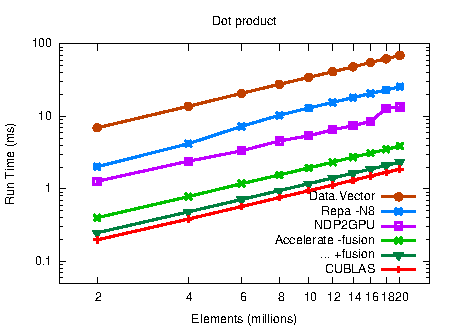
\includegraphics[scale=1.2]{benchmarks/figs/dotp/dotp.pdf}
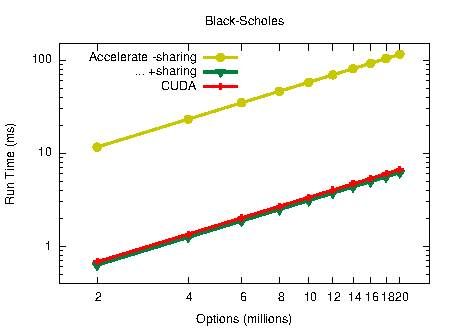
\includegraphics[scale=1.2]{benchmarks/figs/black-scholes/black-scholes.pdf}

\hspace{-1em}
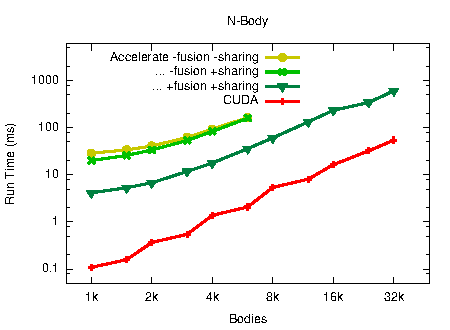
\includegraphics[scale=1.2]{benchmarks/figs/nbody/nbody.pdf}
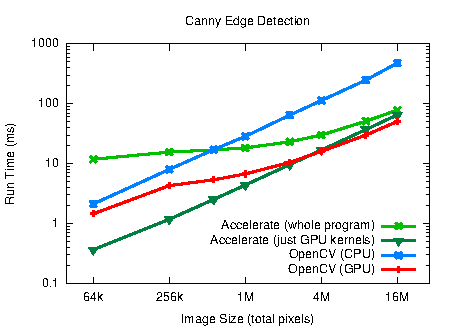
\includegraphics[scale=1.2]{benchmarks/figs/canny/canny.pdf}

\hspace{-1em}
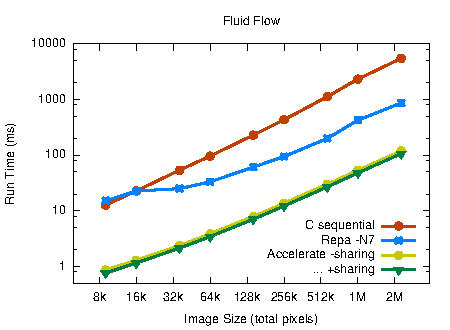
\includegraphics[scale=1.2]{benchmarks/figs/fluid/fluid.pdf}
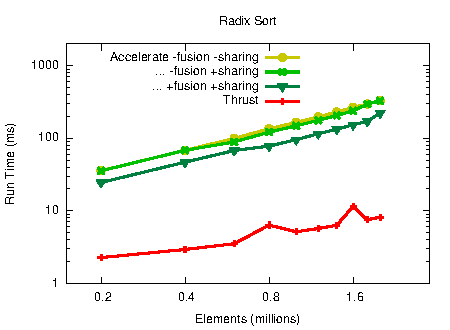
\includegraphics[scale=1.2]{benchmarks/figs/radixsort/radixsort.pdf}
\end{figure*}

% section benchmarks (end)
